\documentclass[18pt]{beamer}
\usepackage[utf8]{inputenc}
\usepackage{xcolor}
\usepackage{hyperref}
\usepackage{templates/mytemplate}
\usepackage{templates/beamerthemekit}
\usepackage{graphicx}
\usepackage{microtype}
\usepackage{listings}
\usepackage{multicol}
\usepackage{siunitx}
\usepackage{physics}
\usepackage{appendixnumberbeamer}
\usepackage{booktabs}
\usepackage{longtable}
\usepackage{amssymb}

\lstset{ %
  backgroundcolor=\color{white},   % choose the background color; you must add \usepackage{color} or \usepackage{xcolor}; should come as last argument
  basicstyle=\tiny\ttfamily,
  xleftmargin=-10pt,
  breaklines=false,                 % sets automatic line breaking
  captionpos=b,                    % sets the caption-position to bottom
  % frame=single,	                   % adds a frame around the code
  keepspaces=true,                 % keeps spaces in text, useful for keeping indentation of code (possibly needs columns=flexible)
  language=C++,                 % the language of the code
  % morekeywords={*,...},            % if you want to add more keywords to the set
  tabsize=2,	                   % sets default tabsize to 2 spaces
  keywordstyle=\bfseries\color{kit-green70},
  commentstyle=\itshape\color{kit-blue70},
  identifierstyle=\color{black},
  stringstyle=\color{kit-orange100},  
}

\hypersetup{colorlinks=true, urlcolor=kit-blue100, %linkcolor=Firebrick4
}

\title{Estimation of the Track Finding Efficiency using Cosmics Data} 
\subtitle{ETP Belle 2 Weekly Meeting}
\author{\underline{Michael Eliachevitch}}
\date{8 November 2018}
\titleimage{transparent}
\institute{ETP -- KIT}


\begin{document}
\selectlanguage{english}

\section{Introduction}
\begin{frame}
  \titlepage
\end{frame}

\begin{frame}
  \frametitle{Overview}
  
\end{frame}

\begin{frame}
  \frametitle{Update on GCR Data and MC}

  \begin{itemize}
  \item use data from Global Cosmic Run (GCR) taken in July 2017
  \item use run numbers 3100--3370 (sugggested by Dong Thang)
    $\Rightarrow$ total 2.8\,Million cosmic events with trigger selecting central tracks\\
  \item also produced 50\,Million cosmic MC events with GCR setup
    \begin{itemize}
    \item same as official MC group: large ``accept box'' of 8\,m $\times$ 8\,m $\times$ 8\,m 
    \item no trigger in simulation, do kinematic cuts on central region ($d_0, z_0$)\\
      $\Rightarrow$  $\sim$10 times less statistics than in data remain
    \end{itemize}
  \end{itemize}

  \begin{block}{Further Information on GCR Data and MC production}
    \begin{itemize}
    \item Data: \footnotesize{\url{https://confluence.desy.de/display/BI/Data+Production+Global+Cosmics+Run+Data\#DataProductionGlobalCosmicsRunData-Runinfo}}
    \item MC: \footnotesize{\url{https://confluence.desy.de/display/BI/Data+Production+Global+Cosmics+Run+MC}}
    \end{itemize}
  \end{block}
  
\end{frame}

\begin{frame}
  \frametitle{Track Parameter Distributions in August GCR and MC}
  \begin{itemize}
  \item August MC samples include trigger simulation
  \end{itemize}
  \begin{center}
    \includegraphics[width=0.35\textwidth]{figures/distributions/gcr_MC_august2017_d0_distribution_uncut.pdf}
    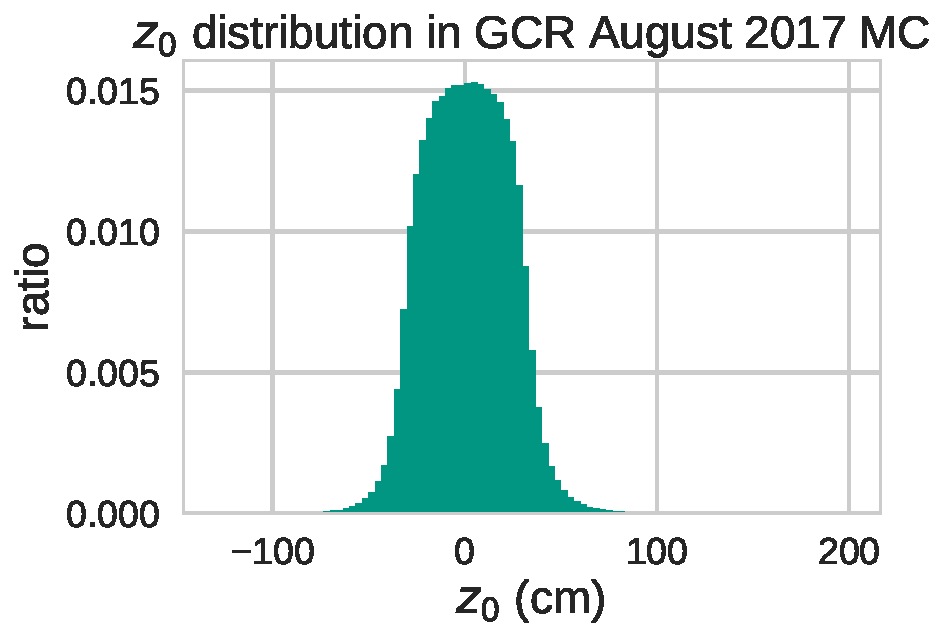
\includegraphics[width=0.35\textwidth]{figures/distributions/gcr_MC_august2017_z0_distribution_uncut.pdf}

    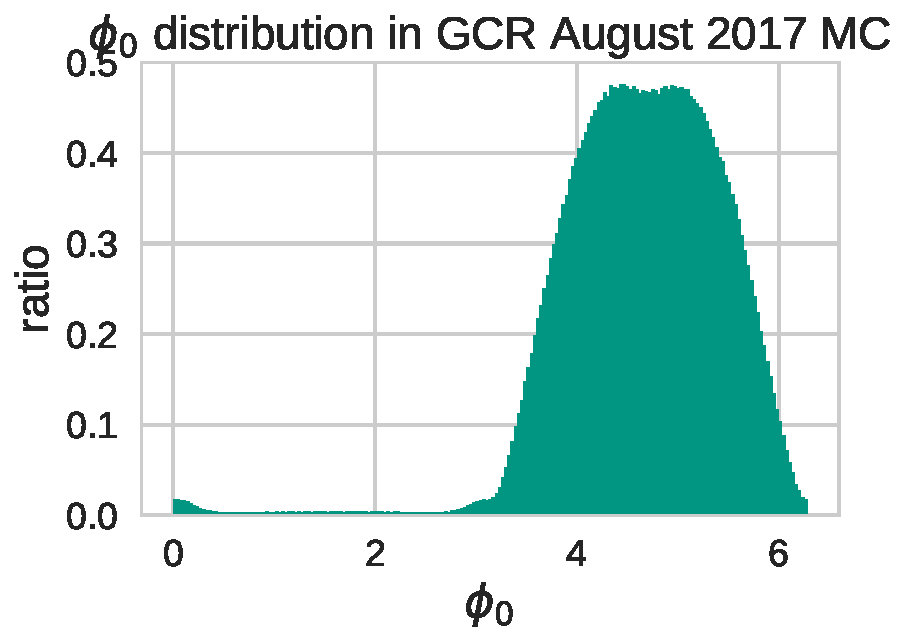
\includegraphics[width=0.35\textwidth]{figures/distributions/gcr_MC_august2017_phi0_distribution_uncut.pdf}
    \includegraphics[width=0.35\textwidth]{figures/distributions/gcr_MC_august2017_tan_lambda_distribution_uncut.pdf}
  \end{center}
\end{frame}

\begin{frame}
  \frametitle{Reminder: Estimation of Finding Efficiency}
  % TODO: insert image of typical cosmic event with trigger
  \begin{itemize}
  \item typical cosmics event: single muon track, no secondaries
  \item cosmics passing through VXD volume create two \texttt{NonMergedRecoTracks}\\
    $\rightarrow$ in the following use those instead of merged \texttt{RecoTracks}
  \item idea: estimate finding efficiency from \textcolor{kit-red100}{finding fails} in events where \textcolor{kit-blue100}{two (findable) tracks are expected}
  \end{itemize}
  \begin{block}{}
    \begin{equation*}
      \label{eq:cosmic_eff}
      \text{Finding efficiency} = \frac{N_\mathrm{2\ tracks\ found}}{\textcolor{kit-blue100}{N_\mathrm{2\ tracks\ expected}}}
      = 1 - \frac{\textcolor{kit-red100}{N_\mathrm{1\ track\ found}}}{\textcolor{kit-blue100}{N_\mathrm{2\ tracks\ expected}}}
    \end{equation*}             %
  \end{block}
  where $N_\mathrm{1\ track\ found}, N_\mathrm{2\ tracks\ found}, \in N_\mathrm{2\ tracks\ expected}$.\\
  
  % \includegraphics[width=0.3\textwidth]{figures/b2display_example_1trackevt_cut.png}
\end{frame}

\begin{frame}
  \begin{center}
    \frametitle{Example Finding Fail Event}
    \includegraphics[width=0.6\textwidth]{figures/b2display_screenshots/b2display_example_1trackevt.png}
    % TODO: Add sketch or annotations
  \end{center}
\end{frame}

\begin{frame}
  \frametitle{Challenges}
    \begin{itemize}
    \item Find a way to select events with two findable track halves, without knowledge of track finder output (prevent bias) $\rightarrow$ other event variables needed
    \item Tracks are not split in MC Track Finder, so we have no MC truth for the number of non-merged reco tracks in the event.
    \end{itemize}
\end{frame}

\section{Necessary steps to get the Finding Efficiency}
\begin{frame}
  \frametitle{Approach: Necessary steps to get the Finding Efficiency}
  
\end{frame}


\begin{frame}
  \frametitle{Split MC Tracks on Hit Distance $c \cdot \Delta t$ to get MC Truth based dataset of two-track-events}
  \begin{itemize}
  \item get distance between hits in \texttt{MCRecoTracks} using timing information of \texttt{CDCSimHit}s
  \item split \texttt{MCRecoTrack} when  $\Delta t$ between \texttt{CDCSimHit}s is larger than some threshold
  \item add new parameter \texttt{SplitAfterDeltaT} to \texttt{TrackFinderMCTruthRecoTracksModule}
  \item \href{https://stash.desy.de/projects/B2/repos/software/pull-requests/737}{pull request} was merged
  \item choose high enough $\Delta t$ to only split tracks when we are sure they passed through VXD volume\\
  \end{itemize}
\end{frame}

\begin{frame}
  \frametitle{Distribution of Maximum CDCHit $\Delta t$} }
  \begin{center}
    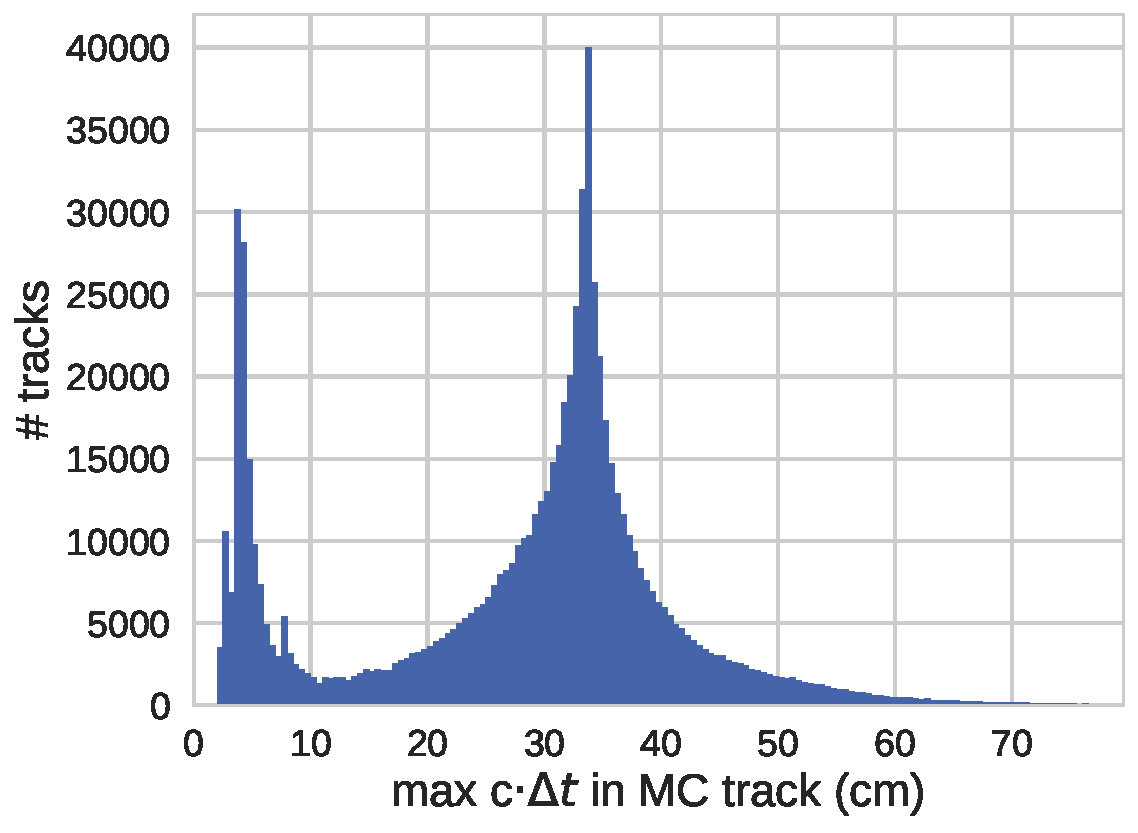
\includegraphics[width=0.8\textwidth]{figures/delta_t/gcraugust_delta_t_max_linear_xmin=0.pdf}
  \end{center}
\end{frame}




\begin{frame}
  \frametitle{Trackfinding-independent selection of expected two-track-events}
  \begin{block}{Select on:}
    \begin{itemize}
    \item Sum of CDCHit y-positions in event, should be near 0 for cosmics creating tracks on top and bottom
    \item Total number of CDC Hits in event
    \end{itemize}
  \end{block}
  Chooce cuts using MC, where
  \begin{itemize}
  \item \textcolor{kit-red100}{one track events}: events with one MC track with hit distances $c\cdot\Delta t < \SI{5}{\cm}$
  \item \textcolor{kit-green100}{two track events}: MC Track has been split on $c\cdot\Delta t > \SI{45}{\cm}$
    and both remaining tracks have only hits with $c\cdot\Delta t < \SI{5}{\cm}$
  \end{itemize}
\end{frame}

\begin{frame}
  \begin{center}
    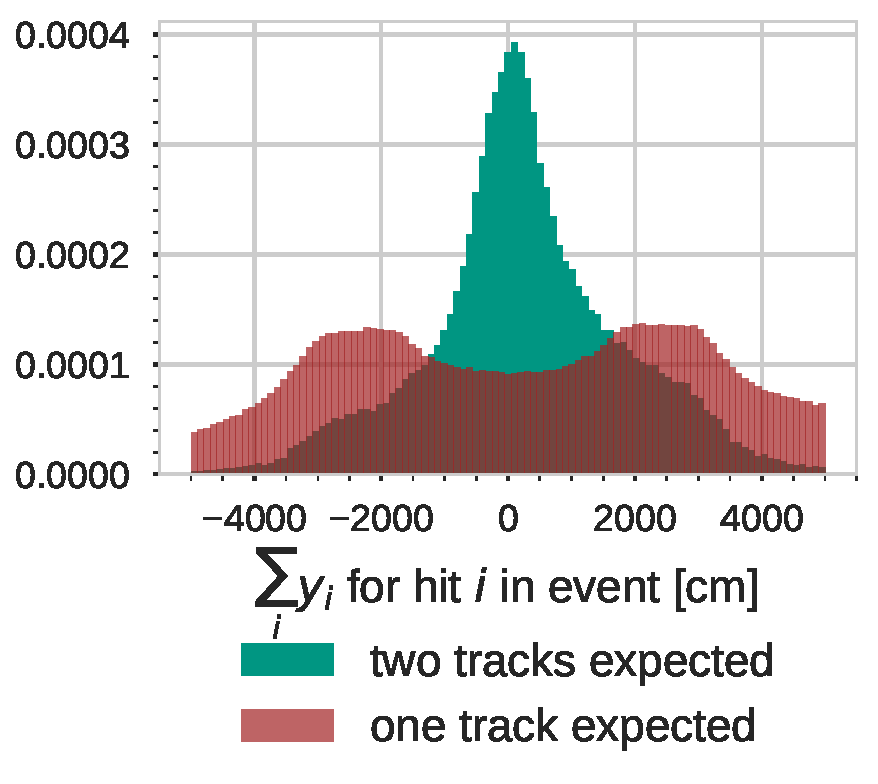
\includegraphics[width=0.44\textwidth]{figures/mcsplit_analysis/sum_y_distribution.pdf}
    \includegraphics[width=0.44\textwidth]{figures/mcsplit_analysis/total_cdc_hits.pdf}    
  \end{center}

  \begin{alertblock}{Choose cut values}
    \begin{itemize}
    \item $85 < \text{number of CDC hits} < 100$
    \item $\abs{\sum{y}} < 400$
    \end{itemize}
  \end{alertblock}
\end{frame}



\begin{frame}
  \frametitle{Distribution of selection parameters for two- and one-track-events from MC datasets from $Delta t$ based selection}
  \begin{center}
    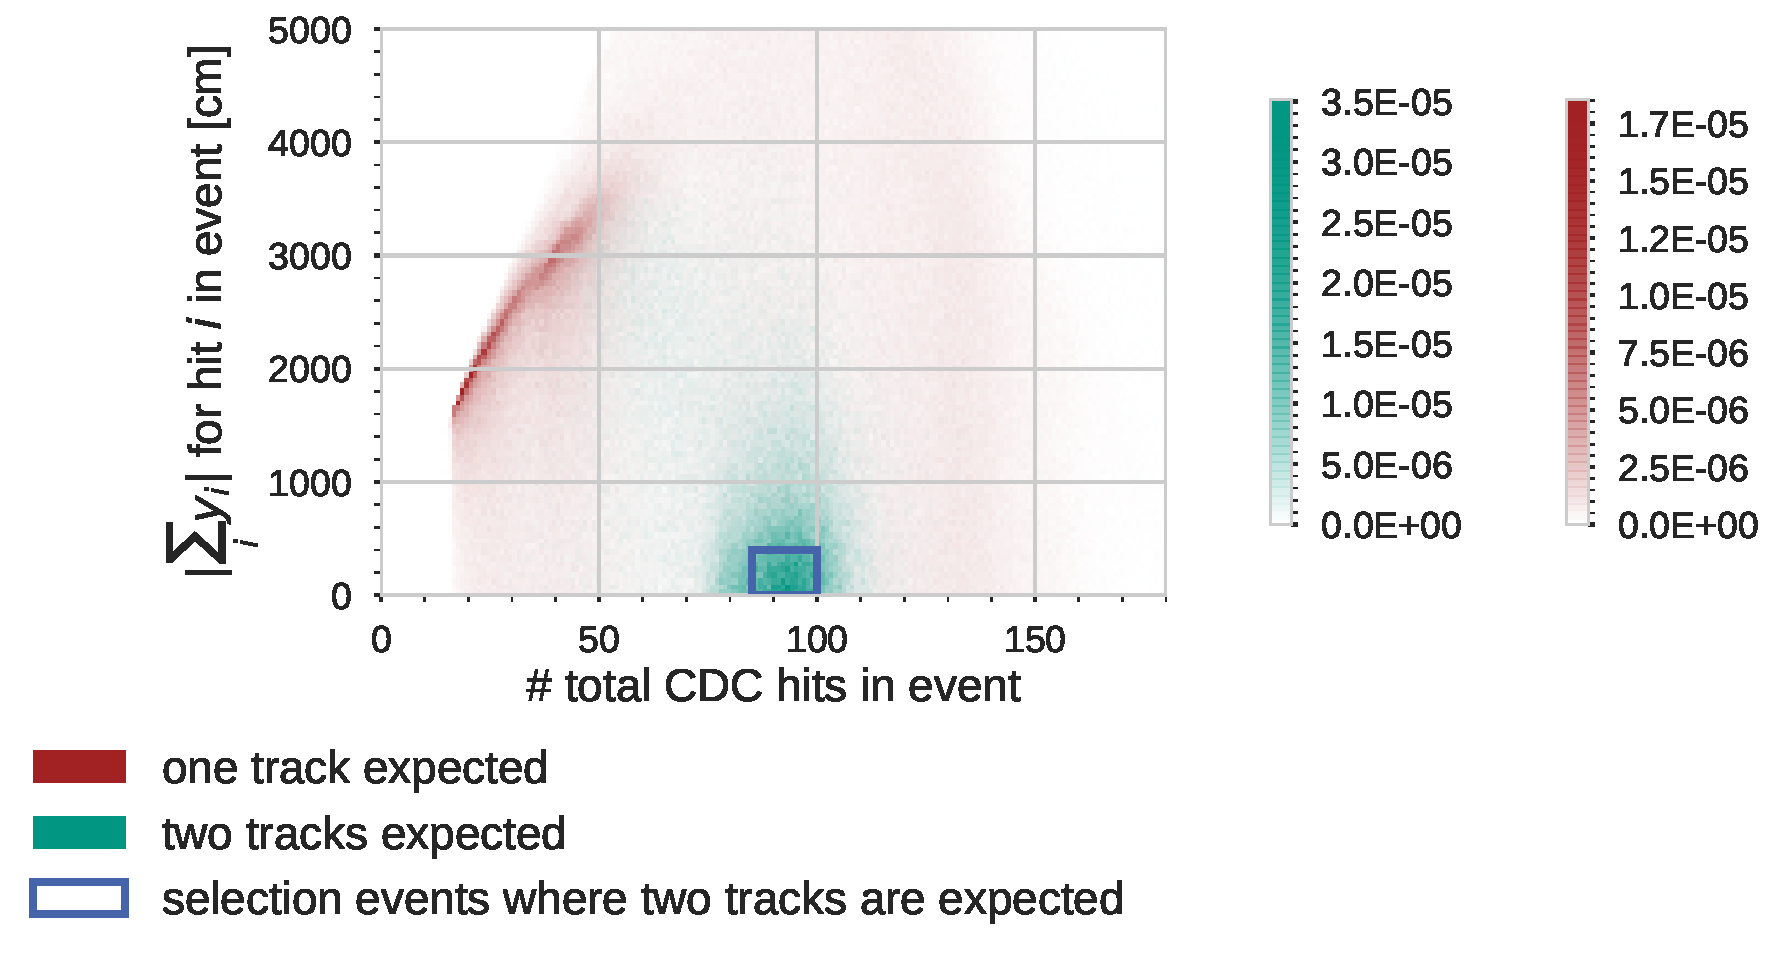
\includegraphics[width=1.0\textwidth]{figures/mcsplit_analysis/sum_y_vs_hits_merged.pdf}
  \end{center}
  \begin{itemize}
  \item 0.7\% of events where we know from MC that one track is expected are in this cut (93\% ``purity'').\\
  \item 14\% efficiency for our MC selection of two track events.
  \end{itemize}
\end{frame}

\begin{frame}
  \frametitle{Event displays in different parameter regions}
  
\end{frame}

\begin{frame}
  \frametitle{Cut away unphysical events based on track parameters?}
  
\end{frame}

\begin{frame}
  \frametitle{Insight: QCS-R visible on $\Delta p_T$ between upper and
    lower track}
  
\end{frame}

\begin{frame}
  \frametitle{Efficiency Plots}
  
\end{frame}

\begin{frame}
  \frametitle{Discussion of my Results}
  
\end{frame}

\begin{frame}
  \frametitle{Outlook}
  
\end{frame}

\section{Backup}
% \backupbegin

\begin{frame}
  \begin{center}
    \huge Backup
  \end{center}
\end{frame}

\begin{frame}
  \frametitle{Kinematic Distributions for Juli GCR}
  \begin{itemize}
  \item plots from GCR July 2017 run
  \item on the left data, on the right MC
  \item no trigger in July MC

  \end{itemize}
  \begin{center}
    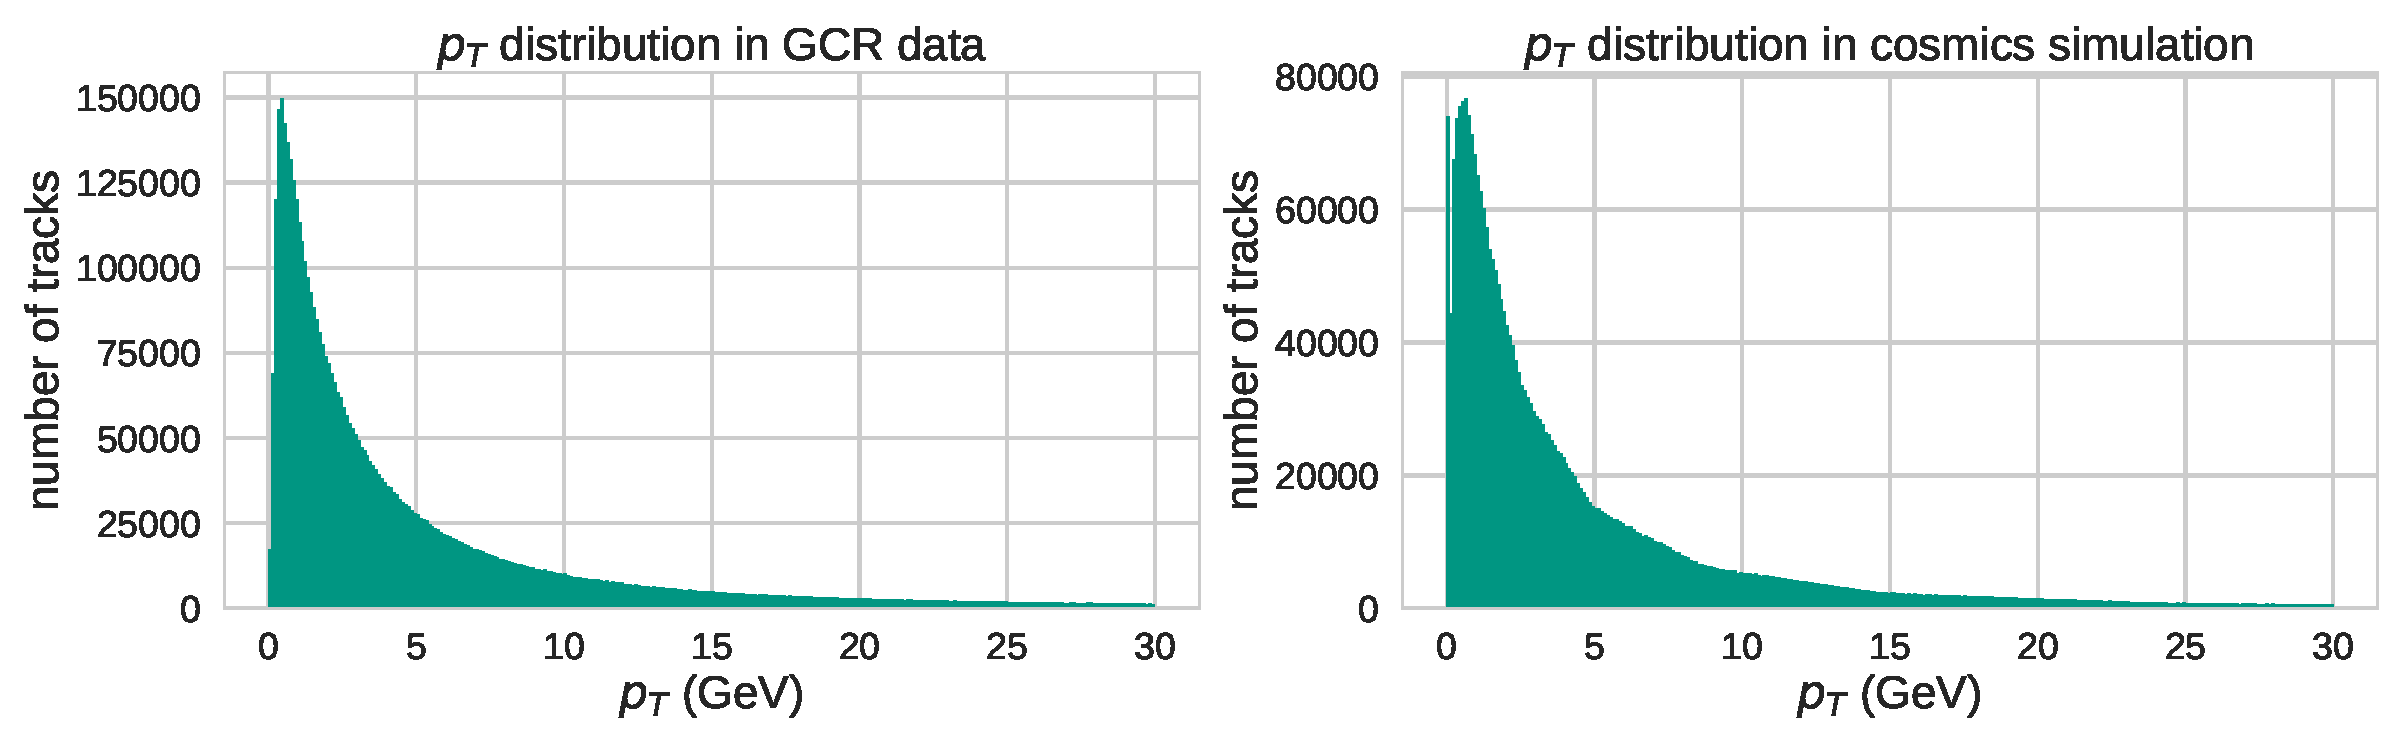
\includegraphics[width=0.8\textwidth]{figures/distributions/gcr_pt_distribution_uncut.pdf}\\
  \end{center}
\end{frame}

\begin{frame}
  \begin{center}
    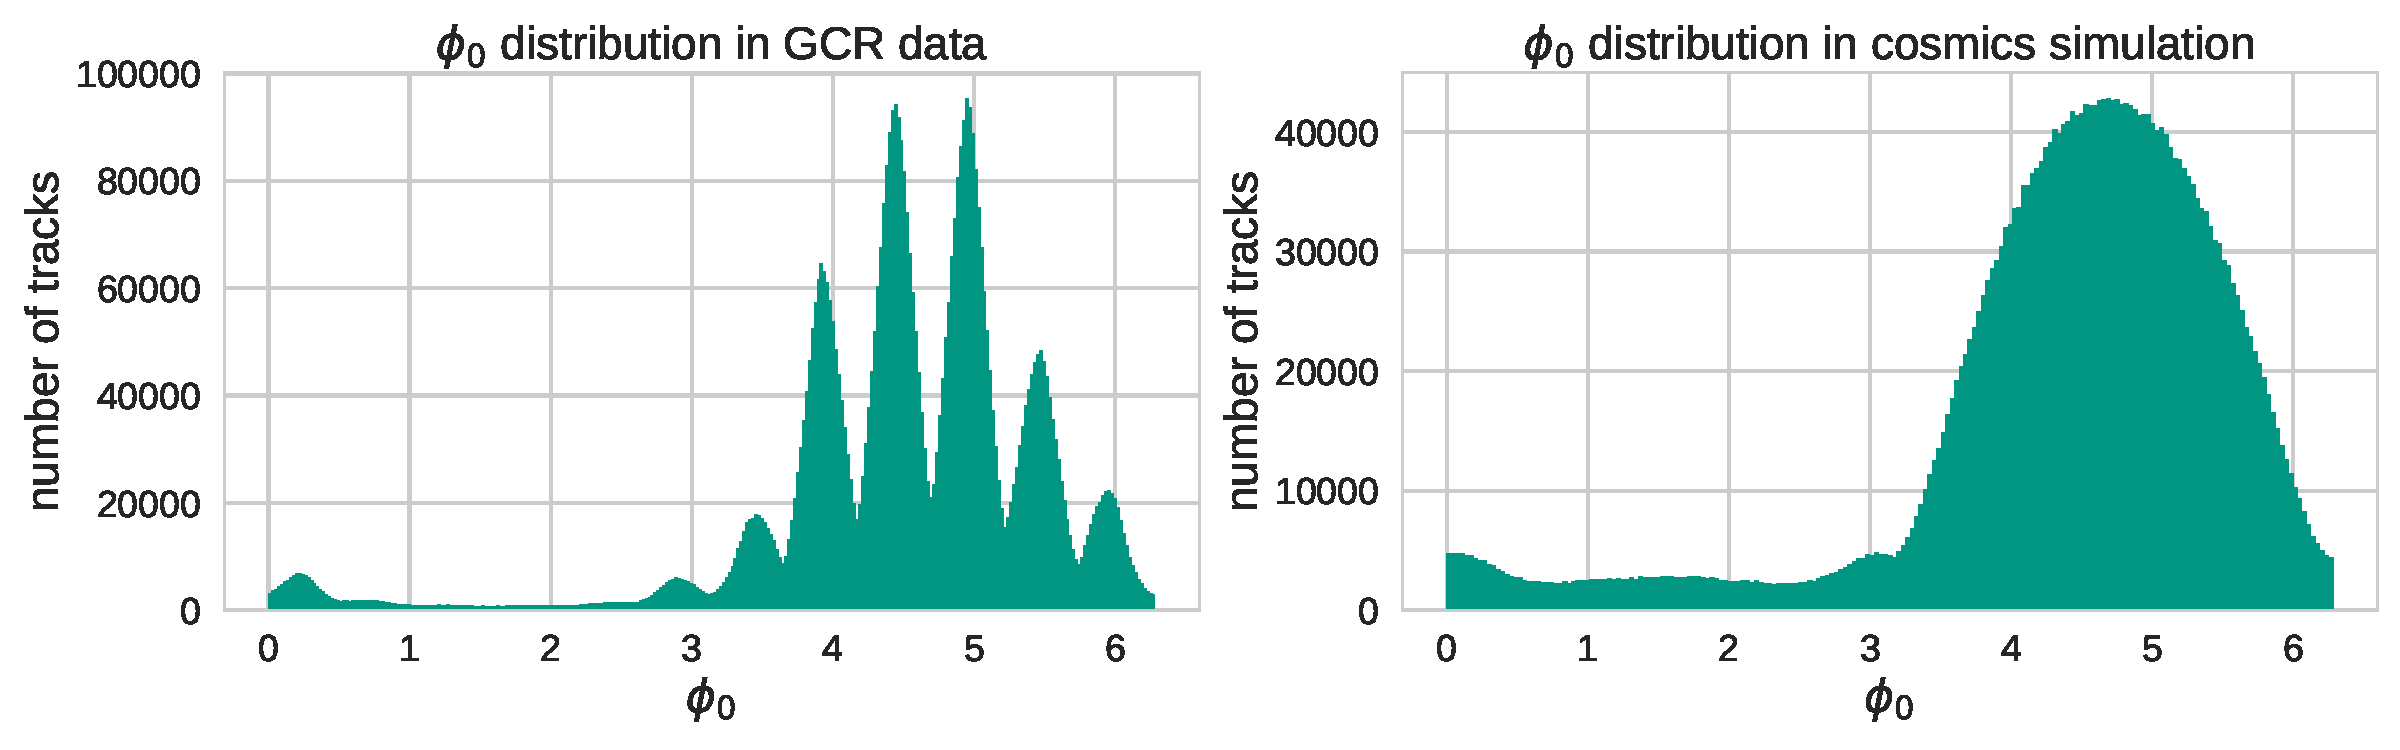
\includegraphics[width=0.8\textwidth]{figures/distributions/gcr_phi0_distribution_uncut.pdf}\\
    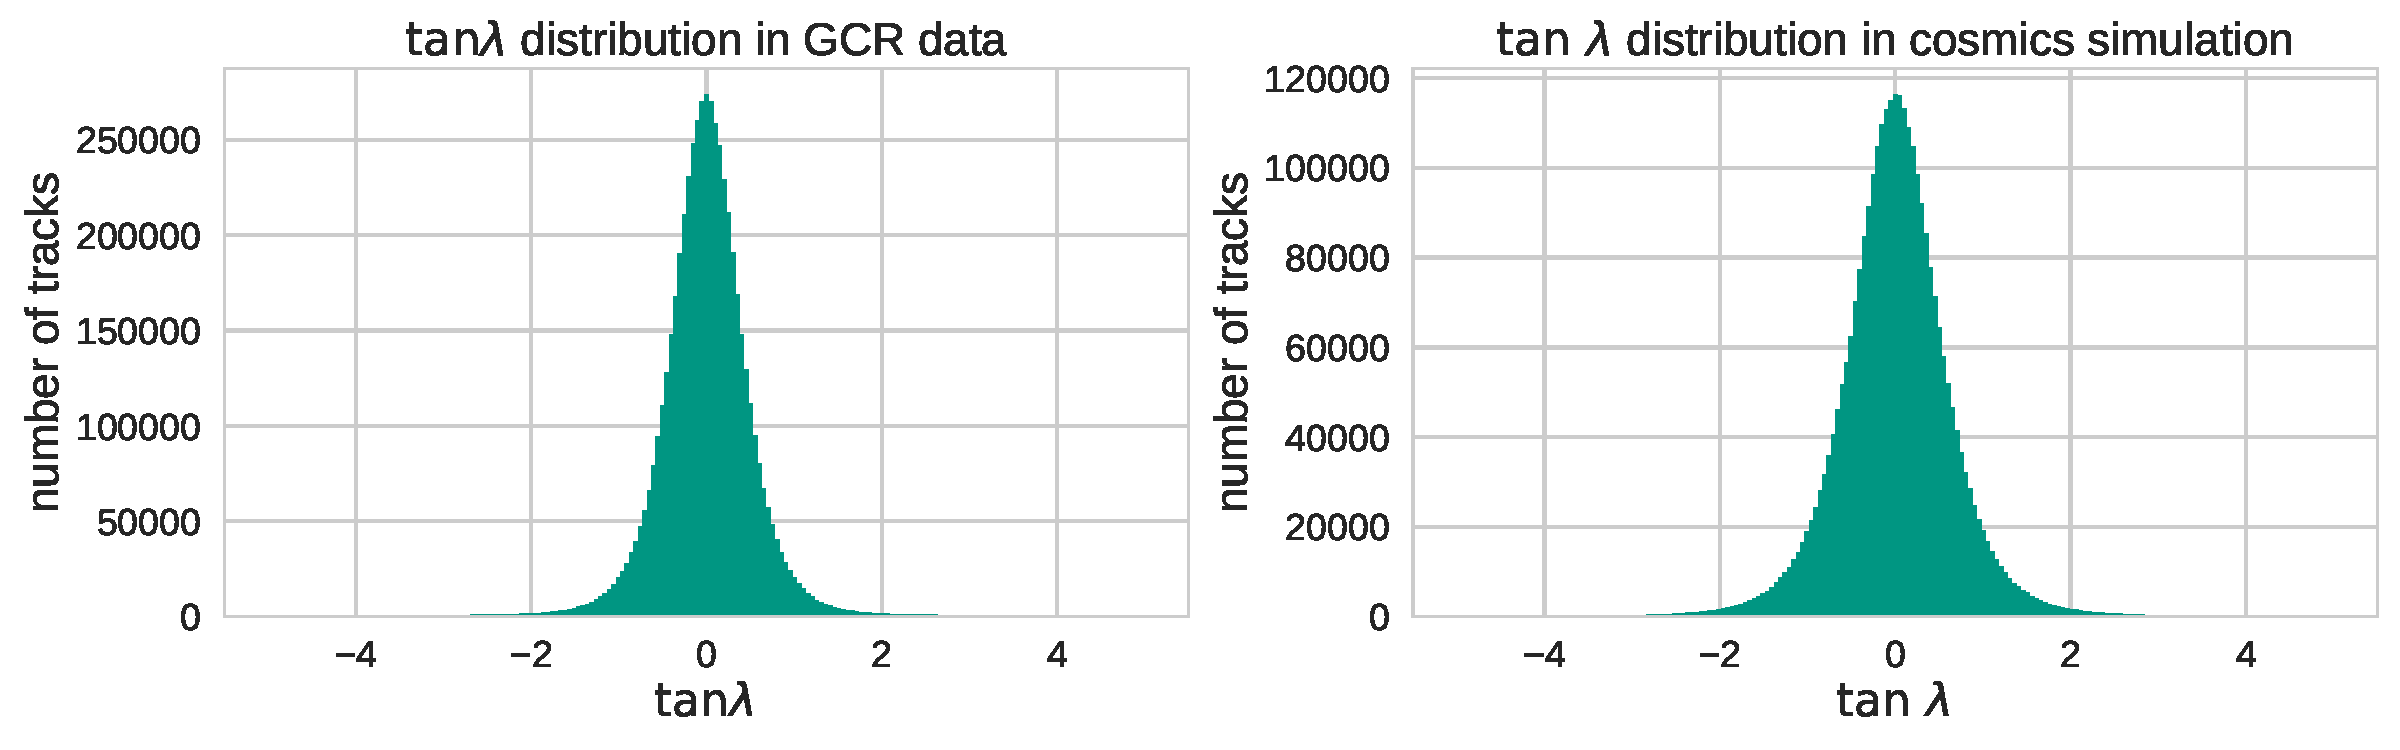
\includegraphics[width=0.8\textwidth]{figures/distributions/gcr_tan_lambda_distribution_uncut.pdf}
  \end{center}
  \begin{itemize}
  \item modulation in $\phi_0$ due to varying trigger efficiencies in July run
  \end{itemize}
\end{frame}

\begin{frame}
  \begin{center}
    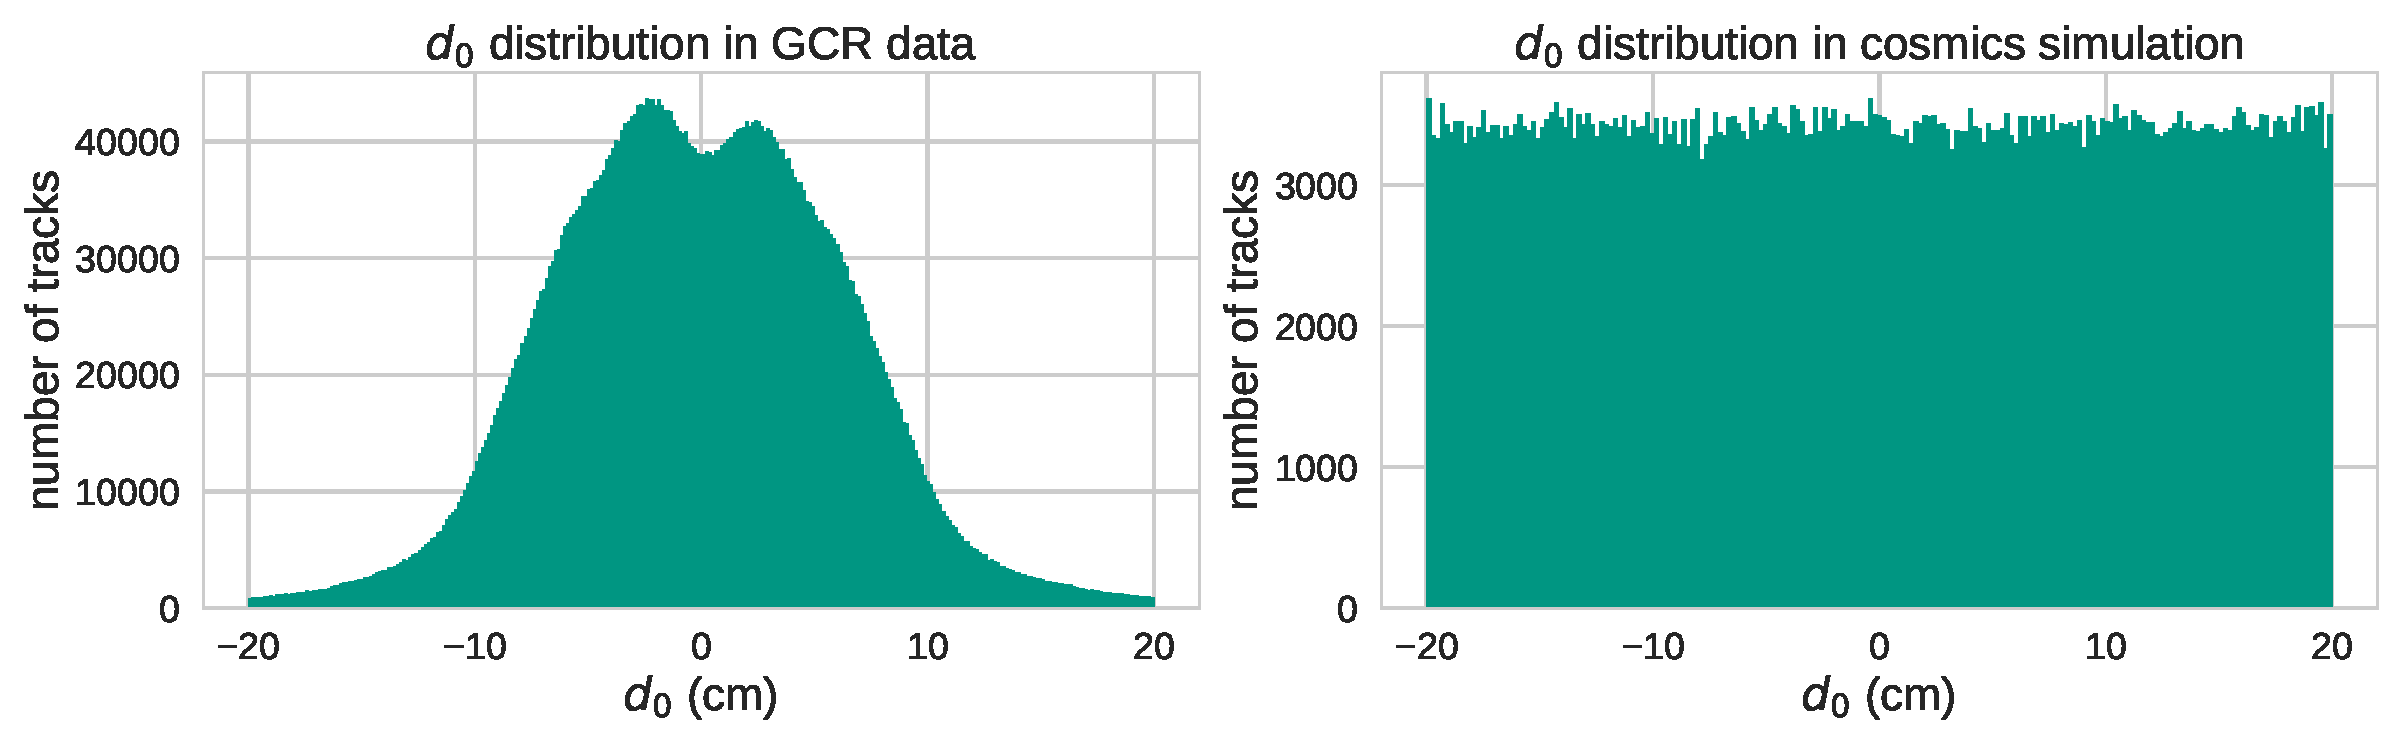
\includegraphics[width=0.8\textwidth]{figures/distributions/gcr_d0_distribution_uncut.pdf}\\
    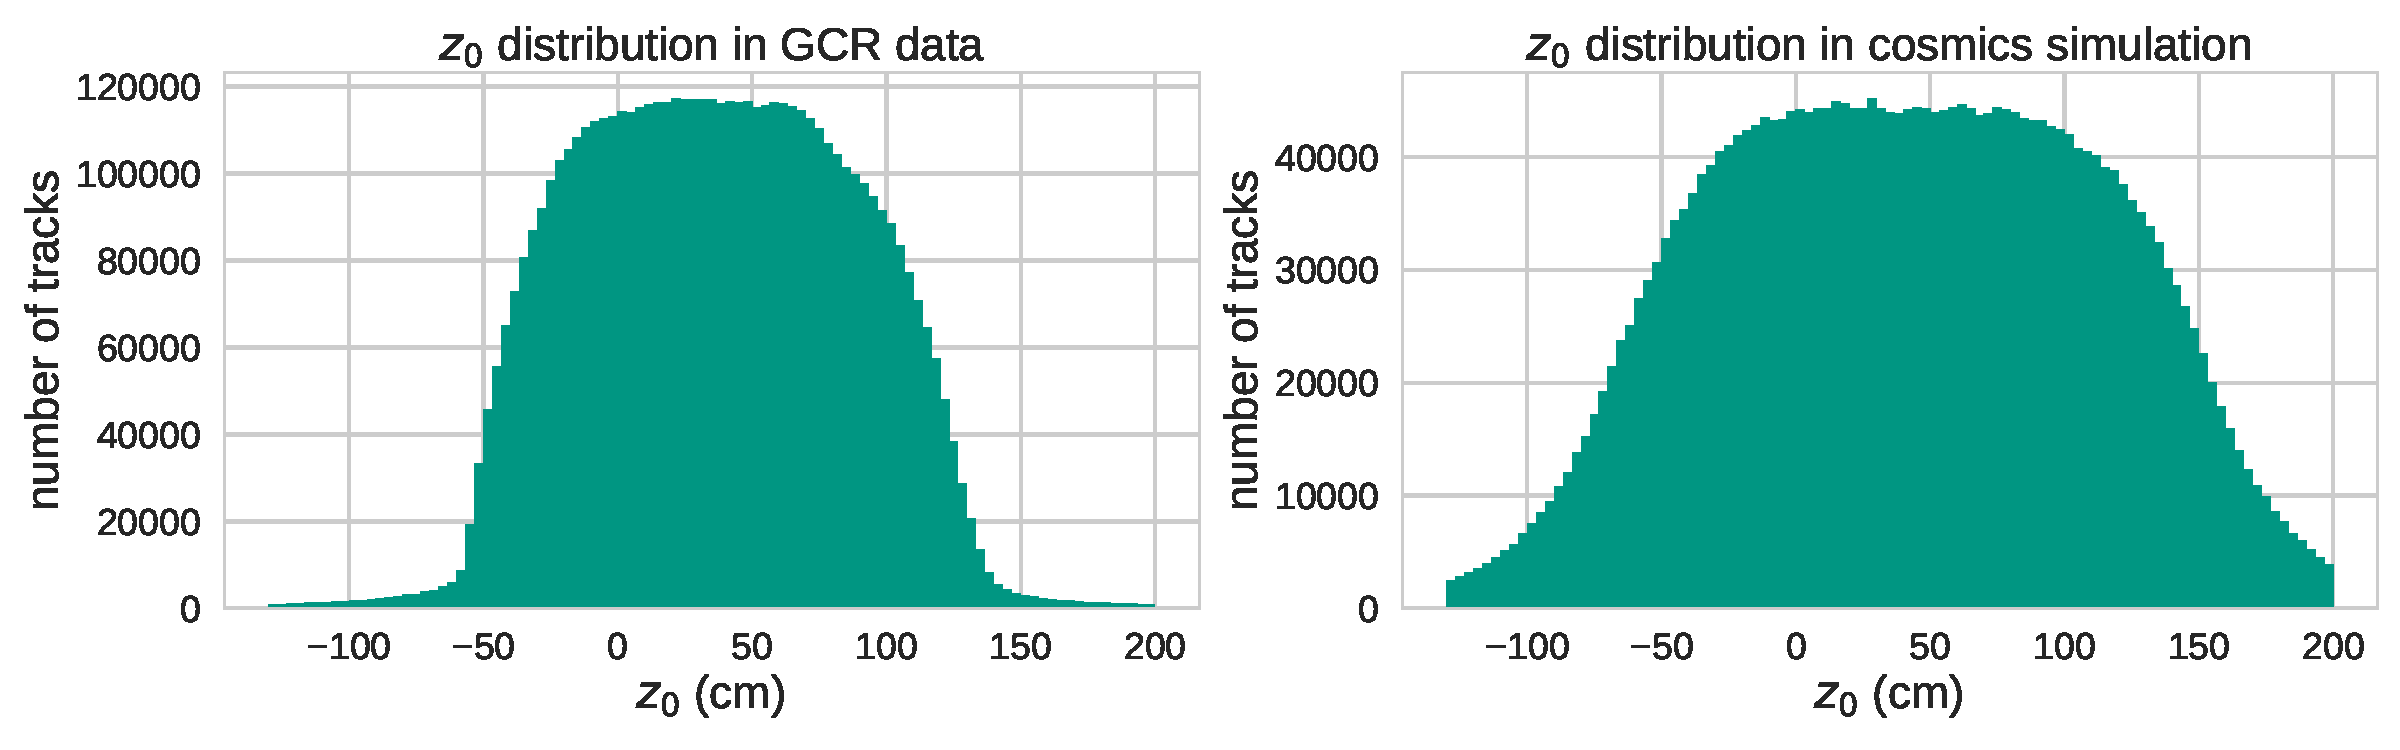
\includegraphics[width=0.8\textwidth]{figures/distributions/gcr_z0_distribution_uncut.pdf}
  \end{center}
\end{frame}

\begin{frame}
  \frametitle{Distribution of Hit $\Delta t$ for all hits in all tracks}  
  \begin{center}
    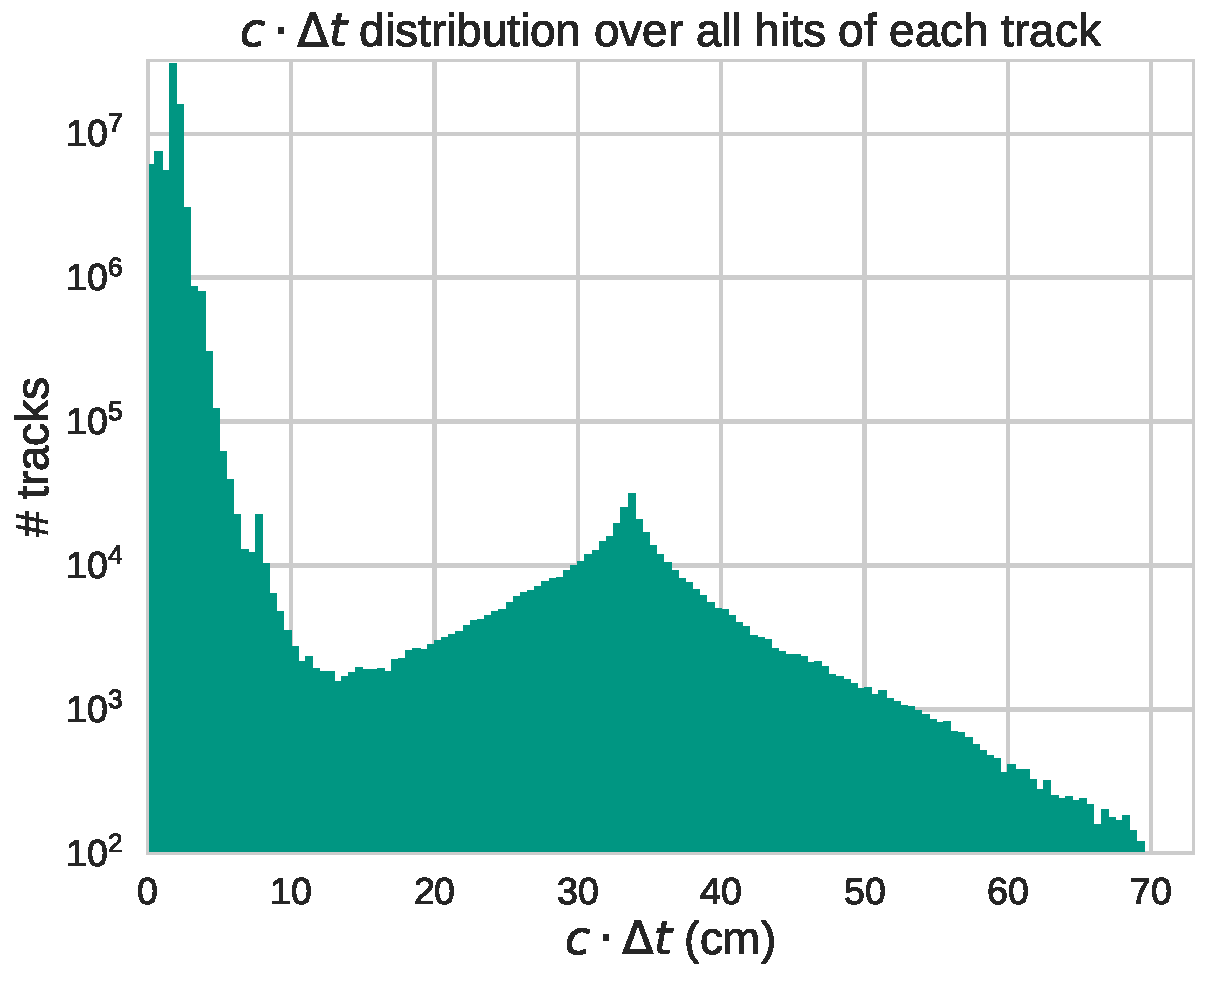
\includegraphics[width=0.45\textwidth]{figures/delta_t/gcraugust_delta_t_log.pdf}
  \end{center}
\end{frame}

\begin{frame}[fragile]
  \frametitle{Code for Splitting Tracks in MC Track Finder}
\begin{lstlisting}[language=C++]
std::vector< std::vector<TimeHitIDDetector> > hitsWithTimeAndDetectorInformationVectors;

if (m_splitAfterDeltaT < 0.0) { // no splitting, vector will only contain a single hitInformation vector
  hitsWithTimeAndDetectorInformationVectors.push_back(hitsWithTimeAndDetectorInformation);
} else { // split on delta t

  std::vector<TimeHitIDDetector>::size_type splitFromIdx = 0; // whenever splitting subtrack, start slice from this index
  for (std::vector<TimeHitIDDetector>::size_type i = 1; i != hitsWithTimeAndDetectorInformation.size(); i++) {

    double delta_t = (std::get<0>(hitsWithTimeAndDetectorInformation[i])
                      - std::get<0>(hitsWithTimeAndDetectorInformation[i - 1]));

    if (delta_t > m_splitAfterDeltaT) {
      // push slice of `hitsWithTimeAndDetectorInformation' between splitFromidx  and previous index
      hitsWithTimeAndDetectorInformationVectors
      .emplace_back(hitsWithTimeAndDetectorInformation.begin() + splitFromIdx,
                    hitsWithTimeAndDetectorInformation.begin() + i);
      splitFromIdx = i;
    }
  }
  // add subtrack after last splitting to list of tracks
  hitsWithTimeAndDetectorInformationVectors
  .emplace_back(hitsWithTimeAndDetectorInformation.begin() + splitFromIdx,
                hitsWithTimeAndDetectorInformation.end());
}
\end{lstlisting}
\end{frame}
% \backupend

\end{document}

%%% Local Variables:
%%% mode: latex
%%% TeX-master: t
%%% End:
